\section{The \sse Platform}\label{sec:platform}

Based on the concepts described in the previous chapter, Chipounov and his team implemented the \sse platform, an open source framework for writing custom system analysis tools.
\sse employs the theoretical concepts of selective symbolic execution by running the system under analysis in a virtual machine and treating code within the scope of interest as symbolic.
These symbolic parts are translated into an intermediate representation (\todo{.}), while irrelevant instructions are directly passed to the host for native execution.


\begin{figure}
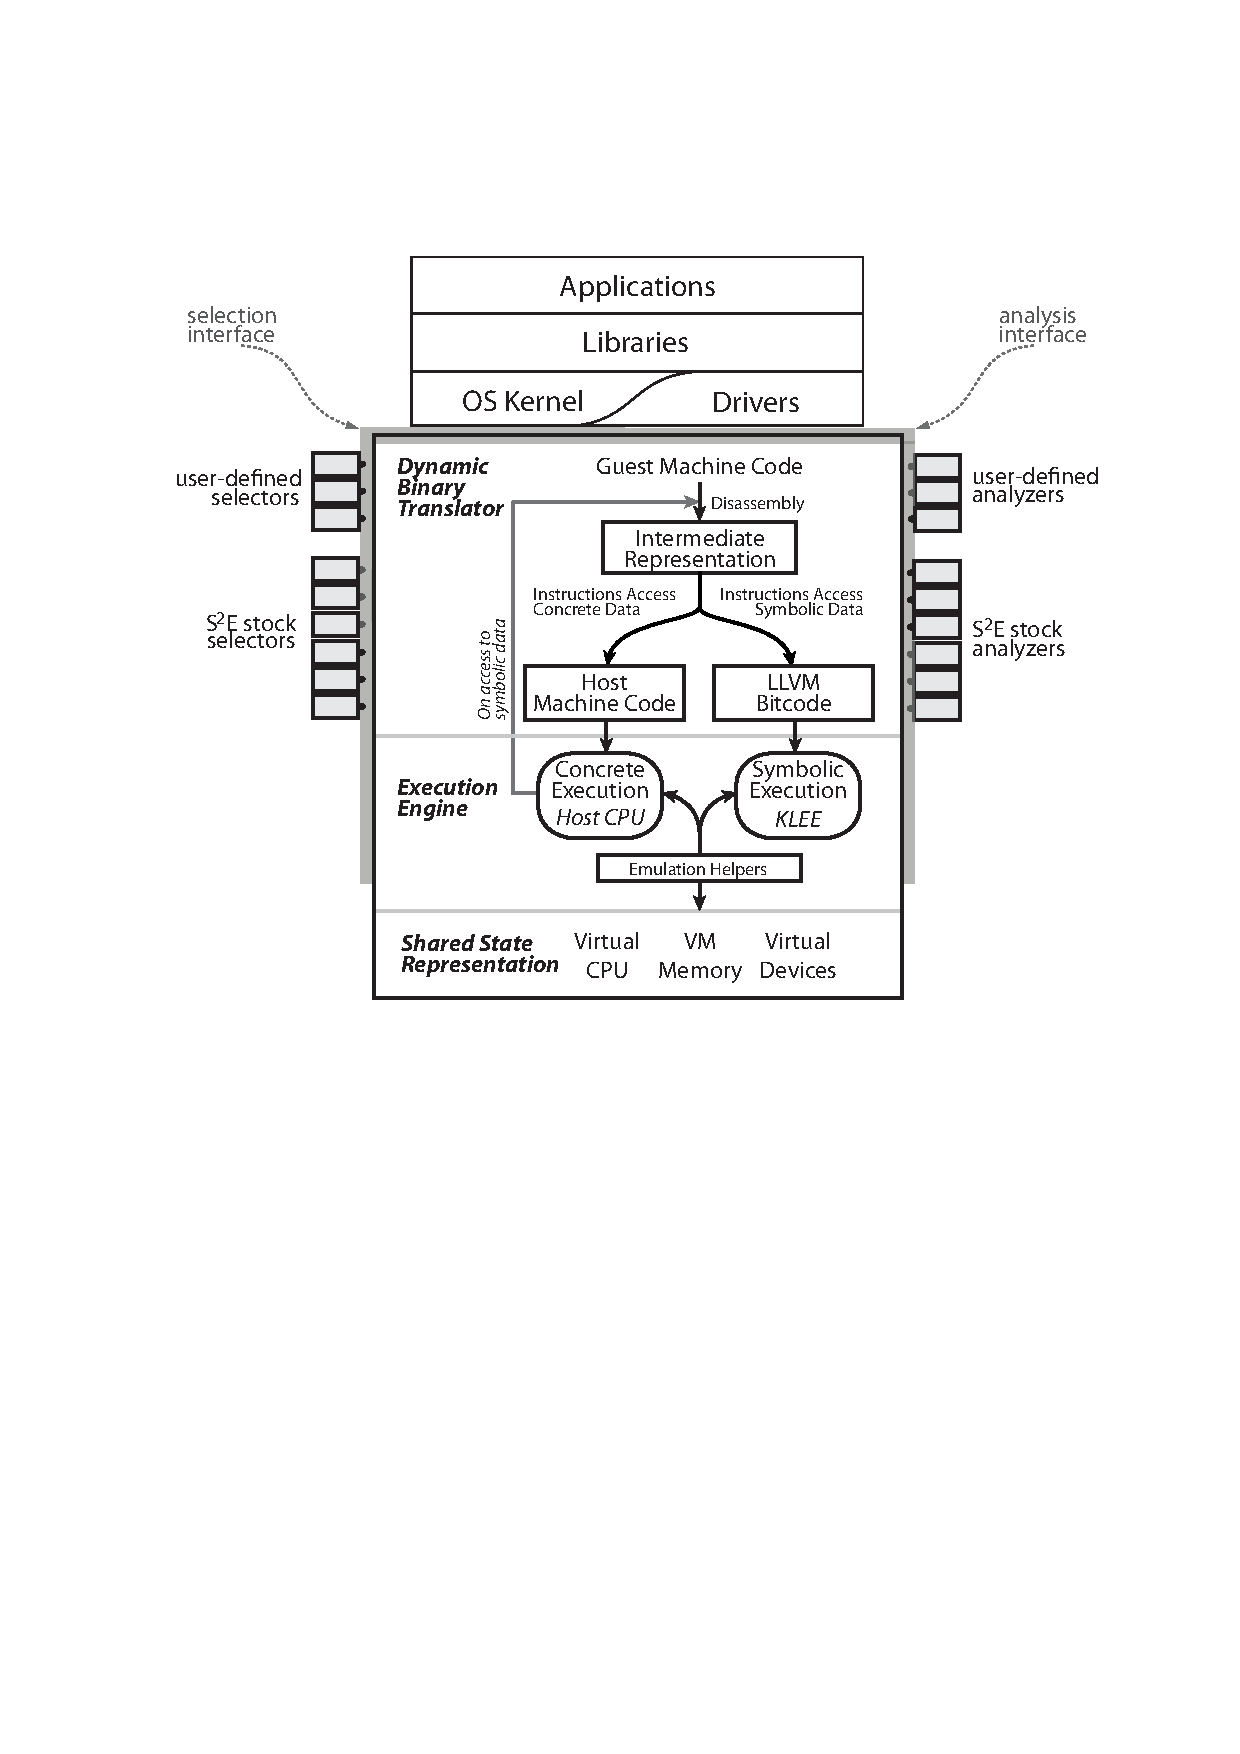
\includegraphics[width=\columnwidth]{s2e_arch}
\caption{Architecture of the \sse platform \cite{chip12s2e}}
\label{fig:arch}
\end{figure}



\iffalse
§3	The S2E Platform
		> Architektur
		> Funktionsweise
		> Selektoren + Analysatoren
\fi